% Source: Code/camera-to-radar_labeller/system_overview.tex
% Description: Busy harbor scenario with 30+ blobs. Harbor entrance contains a dense cluster. Shipping channel has a line of transiting vessels. Scattered blobs appear throughout.

\documentclass[border=4pt]{standalone}
\usepackage{amsmath,amssymb,amsfonts}
\usepackage{tikz}
\usepackage{xcolor}
\usetikzlibrary{arrows.meta,positioning,calc,patterns,decorations.markings,shapes.geometric,fit,backgrounds}

\definecolor{Garnet}{HTML}{73000A}
\definecolor{Rose}{HTML}{CC2E40}
\definecolor{Atlantic}{HTML}{466A9F}
\definecolor{Congaree}{HTML}{1F414D}
\definecolor{Horseshoe}{HTML}{65780B}
\definecolor{Grass}{HTML}{CED318}
\definecolor{Honeycomb}{HTML}{A49137}
\definecolor{Black90}{HTML}{363636}
\definecolor{Black70}{HTML}{5C5C5C}
\definecolor{Black50}{HTML}{A2A2A2}
\definecolor{Black30}{HTML}{C7C7C7}
\definecolor{Black10}{HTML}{ECECEC}
\definecolor{WarmGrey}{HTML}{676156}
\definecolor{Sandstorm}{HTML}{FFF2E3}

\tikzset{
    every node/.style={font=\small},
    sysblock/.style={
        draw=Congaree, fill=Congaree!10, thick,
        minimum width=2.2cm, minimum height=1cm,
        align=center, sharp corners,
        text=black
    },
    sysarrow/.style={
        -Stealth, thick, color=Garnet
    },
    timeblock/.style={
        draw=none, fill=#1, minimum height=0.5cm,
        sharp corners, text=white, font=\footnotesize\bfseries,
        inner sep=2pt
    },
    ppiblob/.style={
        fill=#1, sharp corners, minimum size=4pt, inner sep=0pt
    },
}

\begin{document}
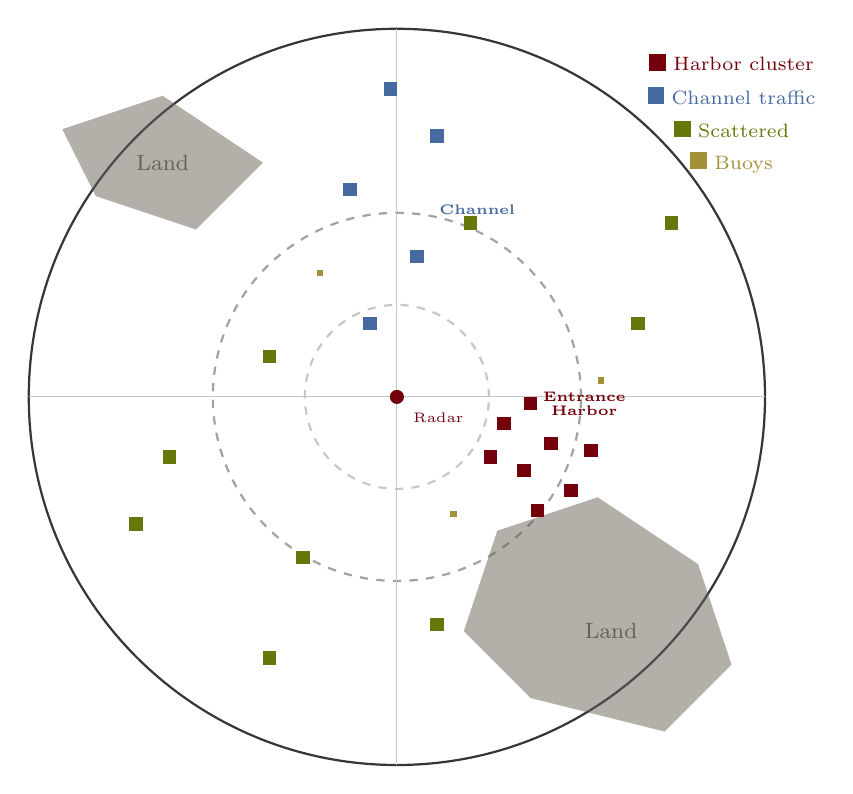
\begin{tikzpicture}[scale=0.85]
    % PPI circle
    \draw[thick, Black90] (0,0) circle (5.5cm);
    \draw[thick, Black50, dashed] (0,0) circle (2.75cm);
    \draw[thick, Black30, dashed] (0,0) circle (1.375cm);

    % Cross hairs
    \draw[Black30] (-5.5,0) -- (5.5,0);
    \draw[Black30] (0,-5.5) -- (0,5.5);

    % Land mass (harbor) -- southeast
    \fill[WarmGrey, opacity=0.5] (1.5,-2) -- (3,-1.5) -- (4.5,-2.5) -- (5,-4) -- (4,-5) -- (2,-4.5) -- (1,-3.5) -- cycle;
    \node[font=\footnotesize, text=WarmGrey] at (3.2,-3.5) {Land};

    % Land mass -- northwest
    \fill[WarmGrey, opacity=0.5] (-3,2.5) -- (-2,3.5) -- (-3.5,4.5) -- (-5,4) -- (-4.5,3) -- cycle;
    \node[font=\footnotesize, text=WarmGrey] at (-3.5,3.5) {Land};

    % Harbor entrance blobs (cluster) -- labeled
    \fill[Garnet] (1.8,-1.2) rectangle (2.0,-1.0);
    \fill[Garnet] (2.2,-0.8) rectangle (2.4,-0.6);
    \fill[Garnet] (1.5,-0.5) rectangle (1.7,-0.3);
    \fill[Garnet] (2.5,-1.5) rectangle (2.7,-1.3);
    \fill[Garnet] (1.9,-0.2) rectangle (2.1,0.0);
    \fill[Garnet] (2.8,-0.9) rectangle (3.0,-0.7);
    \fill[Garnet] (2.0,-1.8) rectangle (2.2,-1.6);
    \fill[Garnet] (1.3,-1.0) rectangle (1.5,-0.8);
    \node[font=\tiny\bfseries, text=Garnet] at (2.8,-0.2) {Harbor};
    \node[font=\tiny\bfseries, text=Garnet] at (2.8,0.0) {Entrance};

    % Shipping channel blobs -- labeled
    \fill[Atlantic] (-0.5,1.0) rectangle (-0.3,1.2);
    \fill[Atlantic] (0.2,2.0) rectangle (0.4,2.2);
    \fill[Atlantic] (-0.8,3.0) rectangle (-0.6,3.2);
    \fill[Atlantic] (0.5,3.8) rectangle (0.7,4.0);
    \fill[Atlantic] (-0.2,4.5) rectangle (0.0,4.7);
    \node[font=\tiny\bfseries, text=Atlantic] at (1.2,2.8) {Channel};

    % Scattered blobs -- unlabeled
    \fill[Horseshoe] (-2,0.5) rectangle (-1.8,0.7);
    \fill[Horseshoe] (-3.5,-1.0) rectangle (-3.3,-0.8);
    \fill[Horseshoe] (-1.5,-2.5) rectangle (-1.3,-2.3);
    \fill[Horseshoe] (3.5,1.0) rectangle (3.7,1.2);
    \fill[Horseshoe] (4.0,2.5) rectangle (4.2,2.7);
    \fill[Horseshoe] (-4,-2) rectangle (-3.8,-1.8);
    \fill[Horseshoe] (0.5,-3.5) rectangle (0.7,-3.3);
    \fill[Horseshoe] (-2,-4) rectangle (-1.8,-3.8);
    \fill[Horseshoe] (1,2.5) rectangle (1.2,2.7);

    % Buoys (stationary, small)
    \fill[Honeycomb] (0.8,-1.8) rectangle (0.9,-1.7);
    \fill[Honeycomb] (-1.2,1.8) rectangle (-1.1,1.9);
    \fill[Honeycomb] (3.0,0.2) rectangle (3.1,0.3);

    % Radar center
    \fill[Garnet] (0,0) circle (3pt);
    \node[font=\tiny, below right, text=Garnet] at (0.1,-0.1) {Radar};

    % Legend
    \node[font=\scriptsize, text=Garnet] at (5.0,5.0) {\rule{6pt}{6pt} Harbor cluster};
    \node[font=\scriptsize, text=Atlantic] at (5.0,4.5) {\rule{6pt}{6pt} Channel traffic};
    \node[font=\scriptsize, text=Horseshoe] at (5.0,4.0) {\rule{6pt}{6pt} Scattered};
    \node[font=\scriptsize, text=Honeycomb] at (5.0,3.5) {\rule{6pt}{6pt} Buoys};
\end{tikzpicture}
\end{document}
